\documentclass[12pt]{article}

\usepackage{sbc-template}
\usepackage[brazil,american]{babel}
\usepackage[utf8]{inputenc}

\usepackage{graphicx}
\usepackage{url}
\usepackage{float}
\usepackage{listings}
\usepackage{color}
\usepackage{todonotes}
\usepackage{algorithmic}
\usepackage{algorithm}
\usepackage{hyperref}
\usepackage{amssymb}
\usepackage{amsmath}
\graphicspath{{../parte1/graficos/}{../parte2/graficos/}}

\sloppy

\title{Trabalho 1\\
Processos Iterativos\\
\& \\
Solução de equações não-lineares}

\author{Dayanne Fernandes da Cunha, 13/0107191\\
       Yurick Hauschild, 12/0024136
}


\address{Dep. Matemática $-$ Universidade de Brasília (UnB)\\
  Cálculo Numérico $-$ Turma A
  \email{dayannefernandesc@gmail.com, yurick.hauschild@gmail.com}
}

\begin{document}
\maketitle

\selectlanguage{brazil}

 \begin{resumo}
 	Este relatório corresponde aos informativos das resoluções do Trabalho 1 de Cálculo Numérico da Turma A do semestre 2016/2.
 \end{resumo}

\section*{Parte I : Processos iterativos}
\label{sec:parte1}

Esta primeira questão será sobre as bifurcações do mapa logístico. Considere o processo iterativo da Equação~\ref{eq:parte1}, chamado de \textit{mapa logístico}. Este processo iterativo, apesar de aparentar ser bastante simples, tem uma dinâmica muito rica, que será analisada em detalhes ao longo desta parte 1 do trabalho.

\begin{eqnarray}
x_{n+1} = \lambda x_{n}(1 - x_{n})
\label{eq:parte1}
\end{eqnarray}

De suas análises, você deve obter que para $\lambda \geq 3$, nenhum ponto fixo é assintoticamente estável. Porém, vamos ver o que acontece quando $\lambda \geq 3$. Já em $\lambda = 3$, você verá que o sistema tem um comportamento interessante: apesar das iterações não convergirem para um ponto fixo, o sistema irá oscilar, depois de algumas iterações, entre dois valores fixos. Quando isto acontece, dizemos que o processo iterativo tem uma \textbf{órbita} de período 2, isto é, $x_{n} = x_{n+2} = x_{n+4} = ... = x_{1}^{*}$ e $x_{n+1} = x_{n+3} = x_{n+5} = ... = x_{2}^{*}$. Este comportamento persistirá até $\lambda \approx 3.449$.

Se aumentarmos um pouco mais $\lambda$, veremos agora que o processo passa a ter órbita de período 4. Se seguirmos aumentando $\lambda$, veremos que o período das órbitas irá dobrar repetidas vezes até $\lambda \approx 3.569$. Isto é o que chamamos de uma bifurcação no sistema e, em particular, esta bifurcação se chama de duplicação de períodos (\textit{period doubling}). O sistema se torna ainda mais rico, porém, se aumentarmos ainda mais $\lambda$. Neste caso, órbitas de qualquer período $k \in  \mathbb{N}$ aparecem, intercaladas com sequências de bifurcações de duplicação de períodos. Isto é o que chamamos de \textit{caos determinístico}. Este comportamento é observado até $\lambda = 4$. A partir deste ponto, as iterações simplesmente divergem.

\subsection*{Questão 1}
\label{sec:p1q1}
Determine analiticamente pontos fixos $x^{*}$ do mapa logístico, Equação~\ref{eq:parte1} e determine as condições para que sejam assintoticamente estáveis. Veja que o parâmetro crucial deste problema é $\lambda$.

\textbf{Resolução:}
A partir do processo iterativo descrito na Equação~\ref{eq:parte1} é possível achar os pontos fixos $x^{*}$ resolvendo a seguinte equação:

\begin{eqnarray}
    \begin{split}
        x^{*} = \lambda x^{*} (1 - x^{*}) \\
        \lambda x^{*} -  \lambda x^{*^{2}} - x^{*} = 0 \\
        x^{*} (\lambda - \lambda x^{*} - 1) = 0
    \end{split}
\label{eq:pto1}
\end{eqnarray}

Pela Equação~\ref{eq:pto1} temos o ponto fixo $x^{*} = 0$. Agora quando $x^{*} \neq 0$:

\begin{eqnarray}
    \begin{split}
        \lambda - \lambda x^{*} - 1 = 0 \\
        - x^{*} = \frac{1 - \lambda}{\lambda} \\
        x^{*} = \frac{\lambda - 1}{\lambda}
    \end{split}
\label{eq:pto2}
\end{eqnarray}

Pela Equação~\ref{eq:pto2} temos o ponto fixo $x^{*} = \frac{\lambda - 1}{\lambda}$.

Para que a Equação~\ref{eq:parte1} do processo iterativo do mapa logístico tenha pontos fixos assintoticamente estáveis é necessário que a condição da dicotomia na Equação~\ref{eq:assest} seja válida para todos os pontos fixos do sistema.

\begin{eqnarray}
    \begin{split}
        g(x^{*}) = \lambda x^{*} (1 - x^{*}) \\
        \left| g'(x^{*}) \right| < 1 \\
        \left| \lambda - 2\lambda x^{*} \right| < 1
    \end{split}
\label{eq:assest}
\end{eqnarray}

Para $x^{*} = 0$, temos:

\begin{eqnarray}
    \begin{split}
        \left| \lambda - 2 \lambda 0 \right| < 1 \\
        \left| \lambda\right| < 1
    \end{split}
\end{eqnarray}

Para $x^{*} = \frac{\lambda - 1}{\lambda}$, por sua vez:

\begin{eqnarray}
    \begin{split}
        \left| \lambda - 2 \lambda \frac{\lambda - 1}{\lambda} \right| < 1 \\
        \left| \lambda - 2 \lambda + 2 \right| < 1 \\
        \left| \lambda - 2 \right| < 1  \\
        \left| \lambda \right| < 3
    \end{split}
\end{eqnarray}

Concluímos, então, que, dado o apropriado $x_{0}$, ${x^{*}}$ vai para 0 com $\lambda < 1$ e para $\frac{\lambda-1}{\lambda}$ com $1 < \lambda < 3$.

\subsection*{Questão 2}
\label{sec:p1q2}
Escreva um programa computacional para calcular os pontos fixos da Equação~\ref{eq:parte1} a partir de seus resultados analíticos e trace um gráfico $\lambda$ x $x^{*}$. Trace, para seis valores representativos de $\lambda$, o resultado das iterações $x_{n}$ x $n$.

\textbf{Resolução:}
Primeiro foi avaliado à escolha do $x_{0}$, que, através da análise do comportamento da função para diferentes valores de $x$, percebeu-se que o intervalo ideal para escolha do $x_{0}$ está contido entre $0.33 < x < 0.5$ como podemos observar na resolução abaixo:

\begin{eqnarray}
    \begin{split}
        0 < g'(x^{*}) < 1 \\
        0 < \lambda - 2 \lambda x < 1 \\
        - \lambda < - 2 \lambda x < 1 - \lambda \\
        \lambda > 2 \lambda x > \lambda - 1 \\
        0.5 > x >  \frac{\lambda - 1}{2 \lambda}
    \end{split}
\end{eqnarray}

Dado que $\lambda < 3$ para o processo iterativo ser assintoticamente estável temos que um $x_{0}$ ideal deve repousar no intervalo $0.33 < x < 0.5$. Escolhemos então o valor $x_{0} = 0.4$.

O algoritmo implementado para gerar os dados do processo iterativo pode ser encontrado no arquivo "$\textit{parte1/questao2.f90}$".

Foram gerados então dois gráficos para demonstrar os resultados analíticos dos pontos fixos, onde, na primeira Figura~\ref{fig:p1q2g1} mostramos o plano cartesiano de $\lambda$ x $x^{*}$ e na Figura~\ref{fig:p1q2g2} é focado nos resultados das iterações $x_{n}$ x $n$.

\begin{figure}[H]
	\centering
	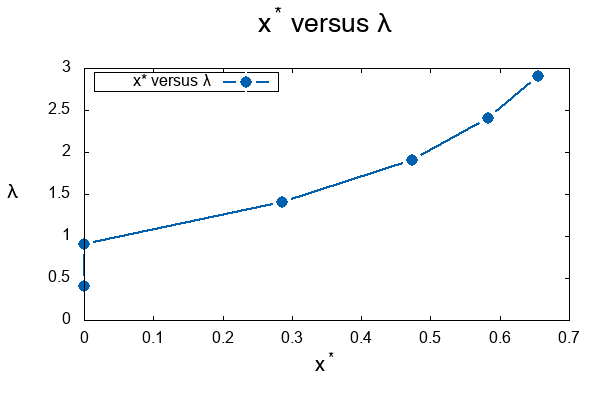
\includegraphics[width=0.6\textwidth]{p1q2g1.png}
	\caption{Gráfico de $\lambda$ versus $x^{*}$.}
	\label{fig:p1q2g1}
\end{figure}

\begin{figure}[H]
	\centering
	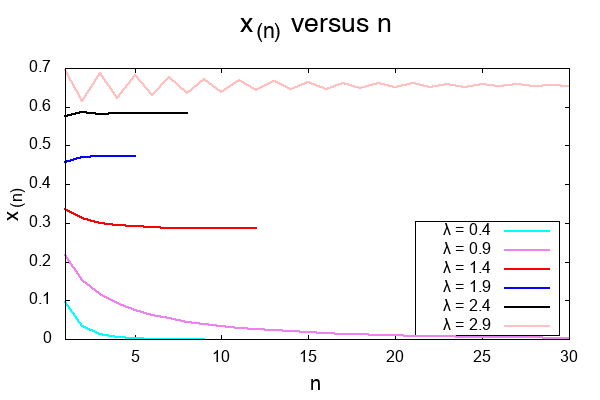
\includegraphics[width=0.6\textwidth]{p1q2g2.png}
	\caption{Gráfico de $x_{n}$ versus $n$}
	\label{fig:p1q2g2}
\end{figure}

\subsection*{Questão 3}
\label{sec:p1q3}
Escreva um programa para determinar, iterativamente, os elementos distintos de suas órbitas para $\lambda$ $\in$ $[3, 4]$, em incrementos de 0.001. Salve os seus resultados em um arquivo e, juntando-os com os pontos fixos encontrados na questão anterior, trace os resultados $\lambda$ x $x_{k}^{*}$, para $\lambda$ variando no intervalo $[0, 4]$, e surpreenda-se com a representação gráfica do caos!

\textbf{Resolução:}
Foi implementado o programa para gerar os dados de $\lambda$ $\in$ $[3, 4]$ em incrementos de 0.001, ele pode ser encontrado no arquivo "$\textit{parte1/questao34.f90}$". Os resultados encontrados podem ser encontrados no arquivo "$\textit{parte1/data/questao3.dat}$". Este arquivo possui na primeira coluna os valores de $\lambda$ entre $[3, 4]$ e nas colunas restantes os valores de cada iteração até formar uma órbita completa para cada valor iterado de $\lambda$.

Traçamos o gráfico $\lambda$ x $x_{k}^{*}$ com os resultados encontrados com o programa desta Questão~\ref{sec:p1q3} e da Questão~\ref{sec:p1q2} variando o $\lambda$ no intervalo $[0, 4]$ e a Figura~\ref{fig:p1q3} foi encontrada. O gráfico encontrado mostra o comportamento oscilatório esperado de $4 \geq \lambda \geq 3$, encontrando bifurcações a partir de $\lambda = 3$.

\begin{figure}[H]
	\centering
	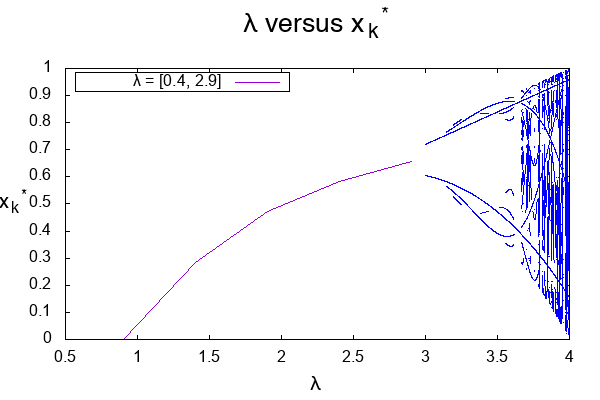
\includegraphics[width=0.6\textwidth]{p1q3.png}
	\caption{Gráfico de $\lambda$ versus $x_{k}^{*}$.}
	\label{fig:p1q3}
\end{figure}

\subsection*{Questão 4}
\label{sec:p1q4}
Para cada valor de $\lambda$ utilizado nos cálculos, salve em uma tabela o período de cada uma das órbitas obtidas e, posteriormente, trace este resultado em um gráfico. Qual é o maior período de uma órbita observada em sua simulação? Quantas vezes a órbita de período 2 foi obtida? E a de período 5?

\textbf{Resolução:}
O algoritmo da Questão~\ref{sec:p1q4} também está contido no arquivo "$\textit{parte1/questao34.f90}$" pois utiliza o mesmo raciocínio. Os dados encontrados através do algoritmo podem ser encontrados no arquivo "$\textit{parte1/data/questao4.dat}$". A primeira coluna da tabela de dados contém valores de $\lambda$ entre $[3, 4]$ em incrementos de 0.001, e na segunda coluna possui o número de períodos de cada órbita de $\lambda$. O gráfico foi gerado a partir desses dados e podemos observá-lo na Figura~\ref{fig:p1q4}. Podemos ver no gráfico que o número de ciclos cresce proporcionalmente à $\lambda$, porém, foi encontrado erros de decaimento nos períodos das órbitas possivelmente devido à erros de aproximação.

O maior período de uma órbita observado na simulação foi de $k = 21$, sendo o $k = 2$ observado em 194 órbitas e $k = 5$ em 13 órbitas.

\begin{figure}[H]
	\centering
	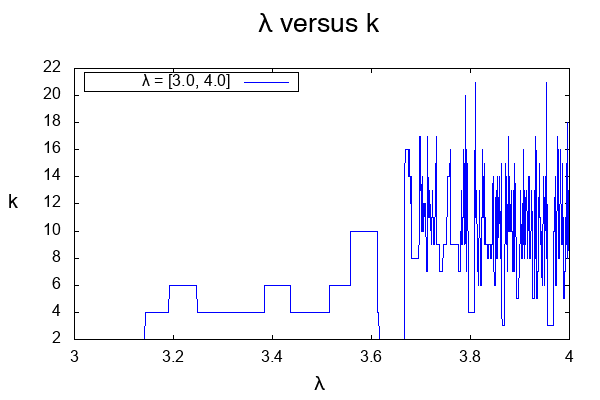
\includegraphics[width=0.6\textwidth]{p1q4.png}
	\caption{Gráfico de $\lambda$ versus $k$.}
	\label{fig:p1q4}
\end{figure}

\section*{Parte II : Solução de equações não-lineares}
\label{sec:parte2}

Nesta segunda parte, vamos estudar o processo de aquecimento de uma barra muito longa de um material, que é aquecida em uma de suas extremidades com o auxílio de um maçarico. Para isto, vamos modelar este processo da seguinte maneira: vamos considerar uma barra de seção transversal constante, semi-infinita e posicionada no eixo $x \leq 0$. A temperatura inicial da barra é $T_{i}$ em toda a barra. O maçarico será modelado especificando-se um fluxo de calor constante $q$ na posição $x = 0$. Considere que a barra tenha difusividade térmica $\alpha$ e que a temperatura da barra seja $T = T (x, t)$. Este problema é governado pela Equação~\ref{eq:parte2} do calor, cuja solução pode ser facilmente encontrada pela aplicação da \textit{Transformada de Laplace} (Equação~\ref{eq:laplace}) (Não é preciso resolver a equação!).

\begin{equation}
\frac{\partial T}{\partial t} = \alpha \frac{\partial^{2} T}{\partial x^{2}} \hbox{, com } \frac{\partial T}{\partial x} (0,t) = q \hbox{ e } T(x,0) = T_{i}
\label{eq:parte2}
\end{equation}

\begin{equation}
T(x, t) = T_{i} + q \left[ 2 \sqrt{\frac{\alpha t}{\pi}} e^{- \frac{x^{2}}{4\alpha t}} - xerfc \left( \frac{x}{2 \sqrt{\alpha t}} \right) \right]
\label{eq:laplace}
\end{equation}

A função $erfc(x)$ é a função erro complementar, definida na Equação~\ref{eq:erfc}.

\begin{equation}
erfc(z) = \frac{2}{\sqrt{\pi}} \int_{z}^{\infty} e^{-w^{2}} dw = 1 - \frac{2}{\sqrt{\pi}} \int_{0}^{z} e^{-w^{2}} dz = 1 - erf(z)
\label{eq:erfc}
\end{equation}

A segunda integral (lado direito) na Equação~\ref{eq:erfc} é a chamada função erro, $erf(z)$. A função $erfc(z)$ é uma função especial, definida por uma integral que não pode ser resolvida explicitamente, já que não há uma primitiva trivial para a função $e^{-z^{2}}$. Porém, sabemos que $erfc(z)$ é uma função decrescente, tal que $erfc(z) \rightarrow 0$ quando $z \rightarrow \infty$ , e que $erfc(0) = 1$. Assim, é fácil perceber o que a Equação~\ref{eq:laplace} representa fisicamente.

A Equação~\ref{eq:laplace} descreve como a temperatura do corpo varia em cada posição $x$ ao longo do tempo $t$. Assim, fixado um $x$, sabemos como a temperatura vai evoluir nesta posição ao longo do tempo. O problema, porém, é que a Equação~\ref{eq:laplace} envolve funções muito complicadas, que não permitem a avaliação direta de valores numéricos. Vamos explorar a Equação~\ref{eq:laplace} computacionalmente e vamos ver o que podemos aprender sobre este sistema. Nesta parte 2 do trabalho, consideraremos que a função erro $erf(z)$ será dada seguinte aproximação racional (\textit{Abramowitz \& Stegun, 1964}):

\begin{equation}
erf(z) = 1 - \frac{1}{(1 + a_{1}z + a_{2}z^{2} + ... + a_{6}z^{ 6 })^{16}}
\label{eq:erf}
\end{equation}

Na Equação~\ref{eq:erf} temos os seguintes valores para as constantes $a1, . . . , a6$:

\begin{align*}
a_{1} = 0.0705230784, \qquad a_{2} = 0.0422820123, \\
a_{3} = 0.0092705272, \qquad a_{4} = 0.0001520143, \\
a_{5} = 0.0002765672, \qquad a_{6} = 0.0000430638. \\
\end{align*}

A função $erfc(z)$ que aparece na Equação~\ref{eq:laplace} deverá ser calculada a partir destas expressões.

\subsection*{Questão 5}
\label{sec:p2q5}
Suponha que queiramos determinar, a partir da Equação~\ref{eq:laplace}, quando a temperatura atingirá um determinado valor especificado $T_{f}$, para valores de $\alpha$, $q$ e $x$ conhecidos. Apresente a formulação para o \textit{Método de Newton-Raphson} aplicado a este problema.

\textbf{Resolução:}
O \textit{Método de Newton-Raphson} é representado da seguinte forma:

\begin{eqnarray}
    \begin{split}
        t_{n+1} = t_{n} - \frac{f(t_{n})}{f'(t_{n})}
    \end{split}
    \label{eq:newr}
\end{eqnarray}

Sendo $f(t_{n})$ e $f'(t_{n}) =\frac{\partial T(x, t)}{\partial t}$ representadas a seguir:

\begin{eqnarray}
    \begin{split}
        f(t_{n}) = T_{i} - T_{f} + q \left[ 2 \sqrt{\frac{\alpha t_{n}}{\pi}} e^{- \frac{x^{2}}{4\alpha t_{n}}} - xerfc \left( \frac{x}{2 \sqrt{\alpha t_{n}}} \right) \right]
    \end{split}
    \label{eq:f(x)}
\end{eqnarray}

\begin{eqnarray}
    \begin{split}
        f'(t_{n}) = \frac{\partial T(x, t_{n})}{\partial t_{n}} = \frac{q \alpha e^{\frac{-x^{2}}{4\alpha t_{n}}}}{\sqrt{\pi \alpha t_{n}}}
    \end{split}
    \label{eq:df(x)}
\end{eqnarray}

Logo aplicando a Equação~\ref{eq:f(x)} e a Equação~\ref{eq:df(x)} no método da Equação~\ref{eq:newr} teremos:

\begin{eqnarray}
    \begin{split}
        t_{n+1} = t_{n} - \left( \frac{T_{i} - T_{f} - qx.erfc \left( \frac{x}{2\sqrt{\alpha t_{n}}} \right) }{\frac{q \alpha e^{\frac{-x^{2}}{4\alpha t_{n}}}}{\sqrt{\pi \alpha t_{n}}}} + 2t_{n}  \right)
    \end{split}
    \label{eq:newrf}
\end{eqnarray}

\subsection*{Questão 6}
\label{sec:p2q6}
Escreva um programa que, para $T_{i} = 10$, $q = 1$ e $\alpha = 1$, determina o tempo $t^{*}$ para que a temperatura em $x = 1$ seja $T_{f} = 50$, usando o método de \textit{Newton-Raphson}. Apresente esta resposta com precisão de 6 casas decimais, indicando quantas iterações foram necessárias para alcançar esta precisão. Faça uma estimativa a priori do chute inicial $t_{0}$, isto é, faça estimativas de valores, justificando seus passos. Apresente, com base no chute inicial, argumentos analíticos para justificar a existência de uma raiz para a equação em questão. Faça um teste da convergência do Método de \textit{Newton-Raphson} em função do chute inicial. Por exemplo, escolha valores para o chute inicial iguais a 2, 3, 4, 5 e 10 vezes o chute estimado no item anterior e compare, num gráfico, a quantidade de iterações necessárias para alcançar a precisão desejada.

\textbf{Resolução:}
O algoritmo da Questão~\ref{sec:p2q6} pode ser encontrado no arquivo "$\textit{parte2/questao6.f90}$". Nele possui o processo iterativo utilizando o método de \textit{Newton-Raphson} apresentado na questão anterior (Questão~\ref{sec:p2q5}) utilizando os valores constantes de $T_{i} = 10$, $q = 1$ e $\alpha = 1$. O arquivo "$\textit{parte2/data/questao6.dat}$" possui o tempo $t^{*}$ encontrado após 5 iterações para quando a temperatura final em $x = 1$ seja $T_{f} = 50$. A resposta é apresentada com uma precisão de 6 casas decimais e foi encontrado utilizando o chute inicial de $t_{0} = 800$.

Analisando a fisionomia de $f(t)$, o chute inicial $t_{0}$ não pode ter valores negativos pois ele está contido dentre raizes quadradas e nem pode ser nulo pois ele tem papel de divisor em alguns termos. Ao utilizar o ponto fixo gerado pelo algoritmo desta questão (Figura~\ref{fig:p2q6g1}) como entrada de $f(t^{*})$ foi obtido como resultado $f(t^{*}) = 0$, o que indica que a raiz encontrada está correta.

\begin{figure}[H]
	\centering
	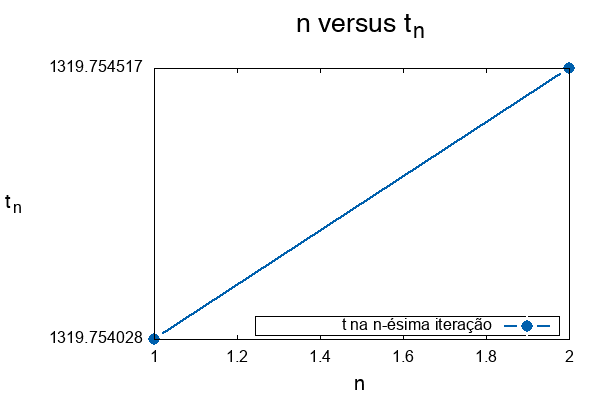
\includegraphics[width=0.6\textwidth]{p2q6g1.png}
	\caption{Gráfico de $n$ versus $t_{n}$.}
	\label{fig:p2q6g1}
\end{figure}

Logo, para verificar a convergência do Método de \textit{Newton-Raphson} utilizamos a dicotomia $\left| f'(t^{*}) \right| < 1$. Quanto mais próximo de 0  $f'(t^{*})$ se aproximar melhor será a convergência, logo, se tivermos $f'(t^{*}) = 0$ teremos uma convergência quadrática. Portanto como podemos ver na Equação~\ref{eq:convnewr} a função irá convergir quase quadraticamente.

\begin{eqnarray}
    \begin{split}
        f'(t_{n}) = \frac{\partial T(x, t_{n})}{\partial t_{n}} = \frac{q \alpha e^{\frac{-x^{2}}{4\alpha t_{n}}}}{\sqrt{\pi \alpha t_{n}}} = \frac{1.1.e^{\frac{-1}{4.1.(1319,754395)}}}{\sqrt{\pi.1.(1319.754395)}} = 1.55273098E-02
    \end{split}
    \label{eq:convnewr}
\end{eqnarray}

A partir do valor inicial de $t_{0} = 100$, pegamos este valor e multiplicamos ele por 2, 3, 4, 5 e 10 vezes para conferir a quantidade de iterações necessárias para alcançar a precisão desejada. O resultado pode ser observado na Figura~\ref{fig:p2q6g2}.

\begin{figure}[H]
	\centering
	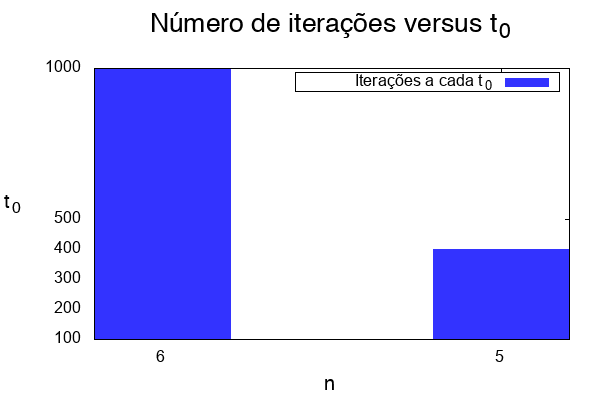
\includegraphics[width=0.6\textwidth]{p2q6g2.png}
	\caption{Gráfico de número de iterações a cada $t_{0}$.}
	\label{fig:p2q6g2}
\end{figure}

\subsection*{Questão 7}
\label{sec:p2q7}
Implemente, também, o método da bisseção para este mesmo problema e, partindo de um intervalo de menor tamanho possível (como escolhê-lo?) centrado no chute inicial da questão anterior, compare a quantidade de iterações necessárias para se alcançar a mesma precisão para $t^{*}$. Mostre como prever este resultado teoricamente.

\textbf{Resolução:}
O método de bisseção foi implementado para o mesmo problema na parte 2 deste trabalho e pode ser encontrado no arquivo "$\textit{parte2/questao78910.f90}$". O intervalo escolhido para aplicar o método foi de $[0, 1600]$

\subsection*{Questão 8}
\label{sec:p2q8}
Para os mesmos valores dos parâmetros $T_{i}$, $q$, $\alpha$, automatize o seu programa para encontrar os valores de $t^{*}$ para posições $x$ variando entre $x = 1$ e $x = 5$. Faça este procedimento para pelo menos 10 pontos neste intervalo, trace um gráfico do seu resultado e comente-o. Você consegue definir uma velocidade da frente de calor que está se propagando por esta barra?

\textbf{Resolução:} O algoritmo implementado para resolver esta questão pode ser encontrado no arquivo "$\textit{parte2/questao78910.f90}$". Para os mesmo valores $T_{i} = 10$, $q = 1$, $\alpha = 1$, buscamos encontrar $t^{*}$ para posições de $x$ variando de $[1, 5]$. Na tabela de dados que se encontra no arquivo "$\textit{parte2/data/questao8.dat}$" contém 10 pontos entre este intervalo sugerido. O gráfico que geramos pode pode ser visto na Figura~\ref{fig:p2q8} abaixo. Podemos analisar pelo gráfico abaixo que ao variar $x$, $t(x)$ cresce proporcionalmente.

A velocidade média de propagação pode ser encontrada utilizando a variação de espaço no tempo, logo, temos a variação de x sendo igual $9$ e a de t igual a $232.753784$, resultando então em $3.86674702E-02$.

\begin{figure}[H]
	\centering
	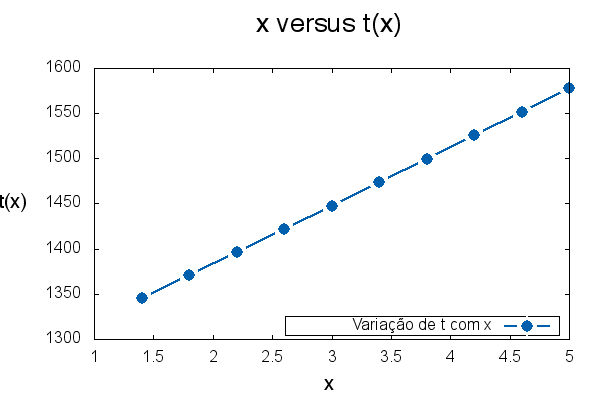
\includegraphics[width=0.6\textwidth]{p2q8.png}
	\caption{Gráfico de $x$ versus $t(x)$.}
	\label{fig:p2q8}
\end{figure}

\subsection*{Questão 9}
\label{sec:p2q9}
Repita o procedimento da Questão~\ref{sec:p2q8}, mas desta vez mantendo-se em um ponto fixo $x$ e variando o valor de $q$ entre $q = 1$ e $q = 10$. Faça este procedimento para pelo menos 10 pontos neste intervalo, trace um gráfico do seu resultado e comente-o. O que acontece quando $q$ aumenta? Agora, faça a mesma análise mantendo-se $q = 1$, mas variando $\alpha$ entre $\alpha = 1$ e $\alpha = 10$. O que acontece quando $\alpha$ aumenta?

\textbf{Resolução:} O mesmo procedimento da Questão~\ref{sec:p2q8} foi seguido e o algoritmo implementado para resolver esta questão também está presente no arquivo "$\textit{parte2/questao78910.f90}$", porém desta vez $x$ está em ponto fixo e temos uma variação de $q$ entra $[1, 10]$. Na tabela de dados que se encontra no arquivo "$\textit{parte2/data/questao9.1.dat}$" contém 10 pontos entre este intervalo sugerido. O gráfico que geramos pode pode ser visto na Figura~\ref{fig:p2q91} abaixo. Podemos analisar pelo gráfico abaixo que ao variar $q$, $t(q)$ varia de forma $e^{-q}$.

\begin{figure}[H]
	\centering
	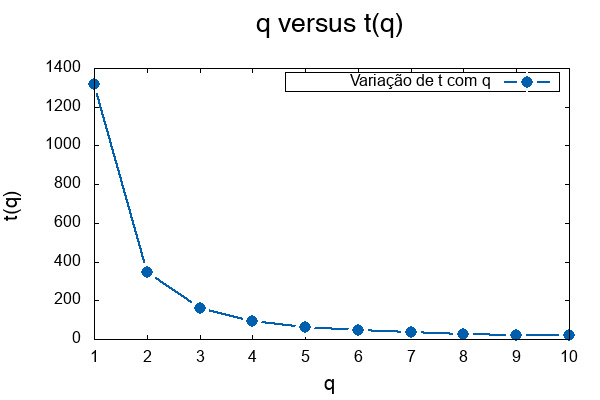
\includegraphics[width=0.6\textwidth]{p2q91.png}
	\caption{Gráfico de variação de $t$ com $q$.}
	\label{fig:p2q91}
\end{figure}

Logo após variamos $\alpha$ entre $\alpha = 1$ e $\alpha = 10$ com ponto fixo de $q = 1$. Na tabela de dados que se encontra no arquivo "$\textit{parte2/data/questao9.2.dat}$" contém 10 pontos entre este intervalo sugerido. O gráfico que geramos pode pode ser visto na Figura~\ref{fig:p2q92} abaixo. Podemos analisar pelo gráfico abaixo que ao variar $\alpha$, $t(\alpha)$ também encontramos a variação da forma $e^{-\alpha}$.

\begin{figure}[H]
	\centering
	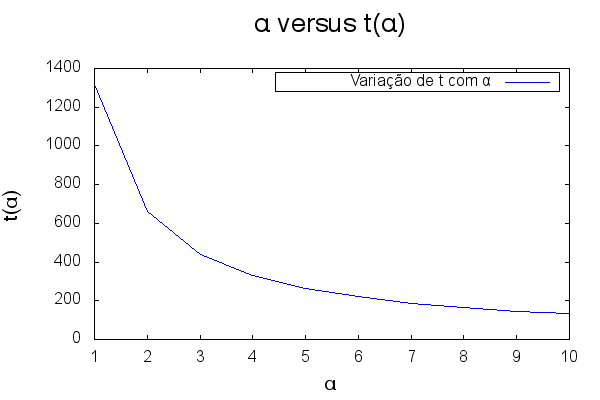
\includegraphics[width=0.6\textwidth]{p2q92.png}
	\caption{Gráfico de variação de $t$ com $\alpha$.}
	\label{fig:p2q92}
\end{figure}

\subsection*{Questão 10}
\label{sec:p2q10}
Que outras análises poderiam ser feitas neste problema e com as ferramentas disponíveis? Escolha uma e apresente seus resultados, comentando-os adequadamente.

\textbf{Resolução:}
É possível verificar o comportamento do processo de aquecimento de uma barra a partir de temperaturas iniciais diferentes. Por exemplo, vamos supor uma variação de $[0, 100]$. Temos como valores fixos $q = 1$, $\alpha = 1$, $x = 1$ e $T_{f} = 500$, sendo assim, o mesmo procedimento da Questão~\ref{sec:p2q8} e  Questão~\ref{sec:p2q9} é utilizado para 10 ponto neste intervalo. Uma tabela de dados foi gerada e o gráfico foi plotado a partir destes dados como podemos analisar na Figura~\ref{}. Podemos analisar que no aumento da temperatura inicial...

\end{document}
